% Please do not change the document class
\documentclass{scrartcl}

% Please do not change these packages
\usepackage[hidelinks]{hyperref}
\usepackage[none]{hyphenat}
\usepackage{setspace}
\doublespace

% You may add additional packages here
\usepackage{amsmath}
\usepackage{graphicx} 
\graphicspath{ {Figures/} }

% Please include a clear, concise, and descriptive title
\title{Are User Stories a Suitable Metric for Burn Down Charts in Agile Game Development?}

% Please do not change the subtitle
\subtitle{COMP150 - Agile Essay}

% Please put your student number in the author field
\author{1507866}

\begin{document}
	
\maketitle
	
\abstract{This essay will analyse the use of user stories in burn down charts in the Agile development process. The focus will be on the use of user stories as a metric in burn down charts and they're suited to use in the games industry.}
	
\section{Introduction}

Kupianinen \textit{et al} say that burn down charts are a measure that should be used by Agile teams \cite{Kupiainen}. The intention of this essay is to look at the use of user stories in burn down charts in the Agile and Scrum development processes. It will also look at whether they are suited to use in games development.

\section{What is the Agile philosophy?}

Agile is a software development method that focuses on the quality of software and finding better ways to develop it \cite{AgileManifesto}. Previously a commonly used software development method was the Waterfall model. This was a sequential process that took place over a series of predefined stages. The clear end to a stage meant that measuring progress in this method was easier than with Agile. \cite{Duka}.

Instead of stages Agile is an iterative process. The development takes place over a series of sprints and during each sprint user stories are completed. User stories are short descriptions from the customer's point of view of a feature that needs to be included in the software. This makes measuring progress in an Agile software development project less clear therefore new metrics are needed for Agile as traditional metrics could be used for Agile but may not give useful data \cite{Misra}.
Scrum is a project management method used alongside Agile. Scrum focuses on customer collaboration with its daily scrum meetings. These meetings are used to discuss who is doing what user story and what the customer wants prioritized \cite{Sutherland}.
There are three main roles in Scrum; the Product Owner, the Scrum Master and the development team. \cite{Ktata}

Agile is suited to use in the games industry as it states in the manifesto that it focuses on responding to change over in depth plans \cite{AgileManifesto}.  Over the development process a game is likely to change a lot. Features may be cut, a certain mechanic may not be fun or an issue arises during play testing. All of these could lead to significant changes in the game. With Agile only the relevant user stories would need to be changed instead of reworking a large design document. Scrum is suited to the games industry as it works with Agile. The daily scrums allow people from different departments to communicate daily and ensure everything is going smoothly.


\section{Metrics}

Metrics are used to quantify software, this could be measuring the development resources or the development process \cite{Misra}. In this essay measuring will refer to progress made in the development process. 

The metrics used should identify and measure areas that will affect the software \cite{Misra}. During software development there are many areas that can be measured however not everything that can be measured should be \cite{Hartmann}.

Another factor to consider when selecting a metric is that the what that metric is measuring will influence the development teams behaviour \cite{Hartmann}. Therefore the metrics should be chosen or  designed to shape the software development process. A poorly designed metric will likely give unhelpful data and not aid development \cite{Ktata}. However a metric that does not aid development may be  Whereas a well designed metric can measure progress but can also aid business decisions and may effect team morale. \cite{Misra}

Another factor affecting metrics is the issue of ``vanity" and ``sanity" metrics. Some metrics may give data that appears impressive but does not give useful data. An example of a ``\textit{vanity}" metric could be time, the metric could be recording how many hours the development team have spent developing the game which could be many hundreds of hours. This metric could give impressive looking results but gives no indication of how many of the games features have been implemented. User stories could be an example of a more useful metric, they could be used to measure how many features have been implemented and how many are left.


\section{Burn Down Charts}
Burn down charts are a common way to measure Agile software development. They are used to record a chosen metric, such as how many user stories were completed in the last sprint \cite{AgileWithScrum}. Velocity can be used in burn down charts to predict an outcome for the given metric. For example how many sprints it will take to complete the project based on how many user stories have been completed in past sprints.

\begin{figure}[h]
	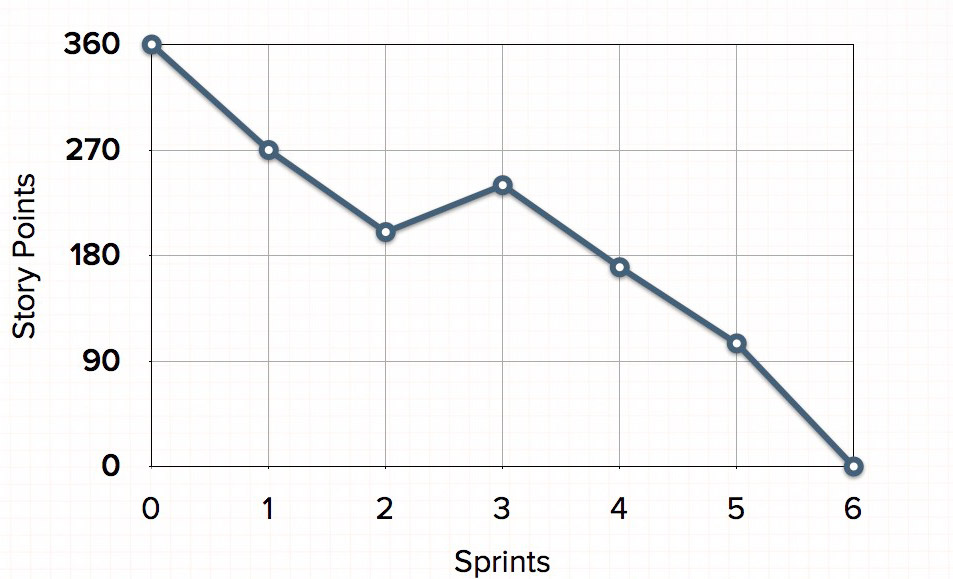
\includegraphics[width=1.0\linewidth]{BDChart.jpg}
	\caption{ An example of a burn down chart \cite{MGS}.}
\end{figure}

Figure 1 above shows an example of a burn down chart. This chart is recording the number of user stories left after each sprint. Velocity could have also been used with this graph to make predictions on how many more sprints would be required to finish all the user stories.

User stories are a metric that could be used in a burn down chart. A simple way to use them would be to record how many user stories are completed in a single sprint. This may work for smaller projects. The issue with this metric is that different user stories may take different amounts of time. Also nearer the end if bugs get put on the backlog this may lead to an invalid velocity.

Ktata and L\'evesque give a list if what factors make a good Agile metric \cite{Ktata}. These factors include having a metric that is easy to collect. User stories are easy to collect, either the number completed or number remaining can be recorded. The metric should also reinforce Agile, user stories are a part of Agile so there use as a metric reinforces their use in the software development.

A potential issue with using user stories as a metric could be that different user stories could take varying amounts of time. This could lead to large changes in the number of user stories completed in a sprint. The predicted velocity would then be invalid. 

An alternative to simply recording the number of user stories is to assign points to each user story and record the number of story points completed in each sprint \cite{Downey}. The points can be based on the priority of user story, the estimated time it'll take to complete or another factor could be chosen \cite{Downey}. A velocity can then be estimated based on how many points are completed per sprint.  This metric could be suitable for the games industry as it would allow user stories from different parts of the game to be prioritized. ... However an issue with this could be that the importance of a user story could be subjective. 


\section{Conclusion}
In conclusion user stories appear to be a suitable metric for use in burn down charts. They provide data that can show the progress being made in Agile game development and can easily be changed as the game evolves.


	
\bibliographystyle{ieeetr}
\bibliography{comp150_agile}
	
\end{document}
